%\graphicspath{{2_modulator/}}  % изменение папки с картинками


\section{Модулятор}

\subsection{Базовая информация о модуляторе}

Задача модулятора - преобразовать поступающие на него данные в сигнал, пригодный для распространения в среде.

Мы рассматриваем системы приёма/передачи цифровых данных, которые описываются следующей схемой (рис.~\ref{system_sch}):

\begin{figure}[h]
\centering
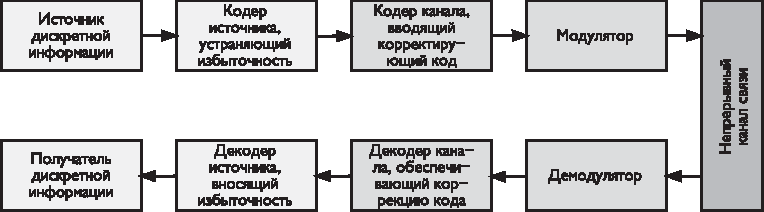
\includegraphics[width = 0.85\textwidth]{system_sch.pdf}
\caption{Блок-схема системы передачи}
\label{system_sch}
\end{figure}

В таких системах модулятор представляет собой блок, который принимает на вход последовательность бит и выдаёт аналоговый радиочастотный сигнал.

Процесс модуляции заключается в изменении одного или нескольких параметров высокочастотной несущей (синусоидального сигнала, генерируемого в передатчике) по закону низкочастотного информационного сигнала (рис.~\ref{simple_mod_sch}).

\begin{figure}[h]
\centering
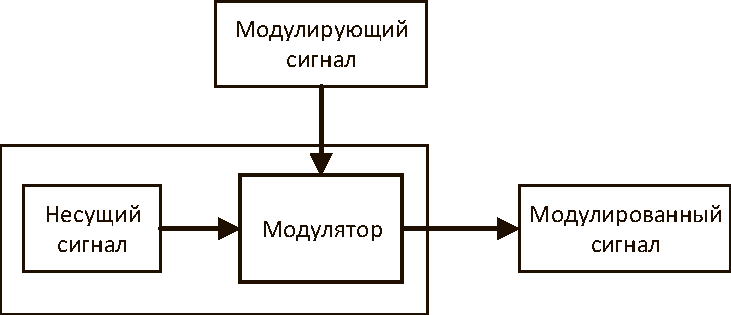
\includegraphics[width = 0.65\textwidth]{simple_mod_sch.pdf}
\caption{Модулятор}
\label{simple_mod_sch}
\end{figure}

Спектр модулированного сигнала на радиочастоте с точностью до постоянного множителя совпадает со спектром модулирующего сигнала, однако центр спектра радиосигнала размещен на несущей частоте, а не на нулевой.

При цифровой полосовой (baseband) модуляции несущее синусоидальное колебание делится на отрезки длиной $T_c$, называемые цифровыми символами, которые отличаются амплитудой, частотой или фазой (или их комбинациями).

В практике передачи цифровой информации чаще всего используется фазовая манипуляция\footnote{цифровую модуляцию часто называют манипуляцией} (PSK) и квадратурная амплитудная модуляция (QAM).		

%%%%%%% схема с квадратурным модулятором




\subsection{Виды}

В простейшем случае модулятор позволяет посылать один сигнал для передачи данных по проводу или беспроводному каналу.
Однако это приводит к неэкономной трате ресурсов (частотных, временных) (в конце концов, намного удобнее использовать один провод, чтобы перенести несколько сигналов, чем проложить отдельный провод для каждого сигнала).
Поэтому были развиты схемы мультиплексирования для совместно использования линий многими сигналами.

\subsubsection{TDM}

При использовании TDM (Time Division Multiplexing, мультиплексирование с разделением времени, временное уплотнение) пользователи сменяются (например, по кругу), и каждый периодически получает всю полосу пропускания на небольшой отрезок времени.

Пример трех потоков, мультиплексированных с помощью TDM, показан на рис.~\ref{tdm}. 
Информационные символы от каждого входного потока взяты в фиксированный временной слот и выведены в совокупный поток.
Этот поток движется с суммарной скоростью отдельных потоков.
Для этого потоки должны быть синхронизированы по времени.
Чтобы компенсировать небольшие отклонения синхронизации, между слотами добавляются маленькие защитные интервалы.

\begin{figure}[h]
\centering
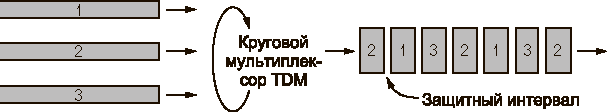
\includegraphics[width = 0.8\textwidth]{tdm.pdf}
\caption{Мультиплексирование с разделением времени (TDM)}
\label{tdm}
\end{figure}

Преимущество TDM состоит в экономном использовании спектра, т.к. для всех сигналов используется одна и та же полоса частот.

Недостатком является то, что скорость передачи мультиплексированного потока обязана быть не меньше (а с учётом наличия защитного интервала - строго больше) суммы скоростей входящих потоков.

TDM широко используется в телефонных сетях и сетях сотовой связи.

\subsubsection{FDM}

В методе FDM (Frequency Division Multiplexing, мультиплексирование с разделением частоты, частотное уплотнение) спектр делится на диапазоны частот, и каждый пользователь получает исключительное владение некоторой полосой, в которой он может посылать свой сигнал.
AM-радиовещание иллюстрирует FDM.
Выделенный спектр составляет приблизительно 1 МГц.
Другие частоты выделены другим логическим каналам (станциям), каждая станция действует в своей части спектра, с межканальным разделением, достаточно большим, чтобы предотвратить помехи.

Более подробный пример на рис.~\ref{fdm} показывает, как три речевых телефонных канала могут объединяться в одну линию с использованием частотного уплотнения.
Фильтры ограничивают используемую полосу частот примерно 3100 Гц на каждый речевой канал.
Когда одновременно мультиплексируется множество каналов, на каждый выделяется полоса 4000 Гц.
Избыток называют защитной полосой, которая сохраняет каналы хорошо отделенными.
Это необходимо, т.к. у реальных фильтров нет идеального резкого края.
Для начала сигналы повышаются по частоте, причем для разных каналов величины сдвигов разные.
После этого их можно суммировать, поскольку каждый канал теперь сдвинут в свою область спектра.

\begin{figure}[h]
\centering
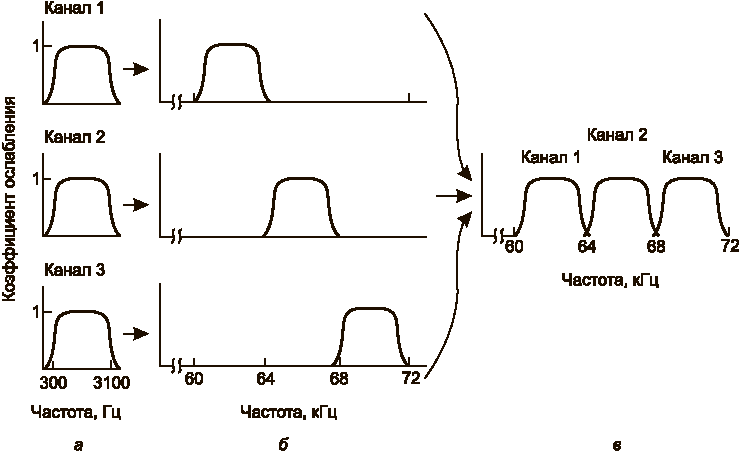
\includegraphics[width = 0.8\textwidth]{fdm.pdf}
\caption{Частотное уплотнение: а — исходные спектры сигналов; б — спектры, сдвинутые по частоте; в — уплотненный канал}
\label{fdm}
\end{figure}

Преимущества и недостатки этой схемы диаметрально противоположны таковым для TDM.
С одной стороны, не требуется временная синхронизация и повышенная скорость выходного потока.
С другой - полоса используемых частот расширяется пропорционально количеству каналов.

Эта схема много лет использовалась для мультиплексирования звонков в телефонной сети, но теперь предпочтение отдается мультиплексированию по времени.
Однако FDM продолжает использоваться в телефонных сетях, а также в сотовых, наземных радио и спутниковых сетях на более высоком уровне разбиения.

%%%%%%%% ИСПРАВЛЕНИЕ %%%%%%%%%%
По сравнению с OFDM (см. следующий раздел), FDM обладает низким пик-фактором, т.е. отношением максимальной мощности к средней мощности.
Таким образом, передатчики с FDM-мультиплексированием не требуют сложных и дорогих усилителей с большой линейной областью в амплитудной характеристике (и большим динамическим диапазоном), а также мощных источников питания.
Поэтому этой схеме мультиплексирования отдается предпочтение в спутниковой связи.
%%%%%%%%%%%%%%%%%%%%%%%%%%%%%%


\subsubsection{OFDM}

При отправке цифровых данных возможно эффективно разделить спектр, не используя защитные полосы.
В OFDM (Orthogonal Frequency Division Multiplexing, мультиплексирование с ортогональным частотным разделением) полоса канала разделена на многие ортогональные поднесущие, которые независимо передают данные (например, с квадратурной амплитудной модуляцией).
Поднесущие плотно упакованы вместе в частотной области.
Таким образом, сигналы от каждой поднесущей простираются в смежные.
%%%%%%%% ИСПРАВЛЕНИЕ %%%%%%%%%%
%Однако, как видно на рис.~\ref{ofdm}, частотная характеристика каждой поднесущей разработана так, чтобы в центре смежных поднесущих это был ноль.
Однако, как видно на рис.~\ref{ofdm}, частотная характеристика каждой поднесущей имеет такую форму, что в центре смежных поднесущих она обращается в ноль.
Это достигается за счёт следующего соотношения между длительностью символа $T_c$ и расстоянием между поднесущими $\Delta f$: $ T_c = \frac{1}{\Delta f}$.
%%%%%%%%%%%%%%%%%%%%%%%%%%%%%%
Поднесущая поэтому может быть выбрана (детектирована) в своей центральной частоте без помех от соседних.
%%%%%%%% ИСПРАВЛЕНИЕ %%%%%%%%%%
%Чтобы это работало, необходим защитный интервал времени, чтобы повторить часть символьных сигналов во времени так, чтобы у них была желаемая частотная характеристика. 
%Однако эти служебные издержки намного меньше, чем при большом количестве защитных полос.
%%%%%%%%%%%%%%%%%%%%%%%%%%%%%%

\begin{figure}[H]
\centering
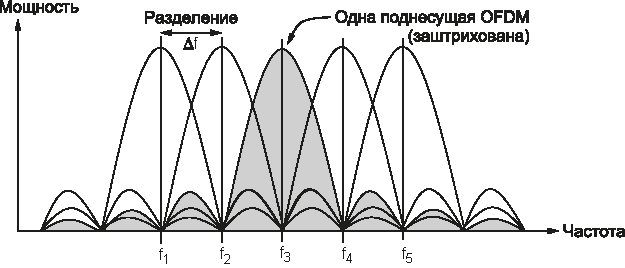
\includegraphics[width = 0.8\textwidth]{ofdm.pdf}
\caption{Мультиплексирование с ортогональным частотным разделением (OFDM)}
\label{ofdm}
\end{figure}

Обычно один высокоскоростной поток цифровой информации разделен на многие потоки с низкой скоростью, которые передаются на поднесущие параллельно.
Это разделение значимо, потому что с дефектами канала легче справиться на уровне поднесущих; некоторые поднесущие могут быть очень ухудшены и исключены в пользу поднесущих, которые принимаются хорошо.

Идея OFDM существовала уже давно, но только в последние десятилетия она стала широко распространена, после того как стало возможно осуществить OFDM эффективно с точки зрения преобразований Фурье цифровых данных по всем поднесущим (вместо того, чтобы отдельно модулировать каждую поднесущую).
OFDM используется в стандартах 802.11 (WiFi), системах цифрового телевещания DVB, мобильных сетях LTE, в системе РАВИС.


\subsection{Модулятор OFDM}

OFDM позволяет эффективно использовать спектр выделенной полосы частот, а также бороться с неблагоприятными условиями воздействия помех в канале связи, к которым наряду с гауссовским шумом относятся замирание сигнала, интерференция, многолучевое распространение сигналов.

OFDM-сигнал может рассматриваться как множество медленно модулируемых узкополосных сигналов, а не как один быстро модулируемый широкополосный сигнал.
Низкая символьная скорость делает возможным использование защитного интервала между символами, что позволяет справляться с временным рассеянием и устранять межсимвольные искажения.

Принцип OFDM-модуляции заключается в следующем.
%%%%%%%%%%%%%% ИСПРАВЛЕНИЕ %%%%%%%%%%%%%%
%В полосе канала связи передается множество несущих, каждая из которых модулируется (например, с использованием QAM-модуляции) частью общего цифрового потока.
В полосе канала связи передается множество несущих, часть из которых (активные несущие) модулируется (например, с использованием QAM-модуляции) частью общего цифрового потока. Все остальные несущие (пассивные) --- это пилотные и пустые несущие. 
%%%%%%%%%%%%%%%%%%%%%%%%%%%%%%%%%%%%%%%%%%
До преобразования спектра такого сигнала цифровой поток разбивается на последовательности, каждая из которых соответствует передаче $kR_a$ битов информации, где $R_a$ --- число активных несущих, $k$ --- коэффициент используемой QAM-модуляции (или число битов информации, передаваемой на каждой активной несущей).
Длительность $T_0$ интервала, на котором передаются все указанные $kR_a$ битов информации, определяет минимальную частоту несущей $f_U = 1/T_U$ и интервал между несущими, т. е. частотный интервал $(R_a + R_n)f_U$, где $R_n$ --- число пассивных несущих, характеризует групповой спектр мощности радиосигнала.

\subsubsection{Схема работы}

\begin{figure}[h]
\centering
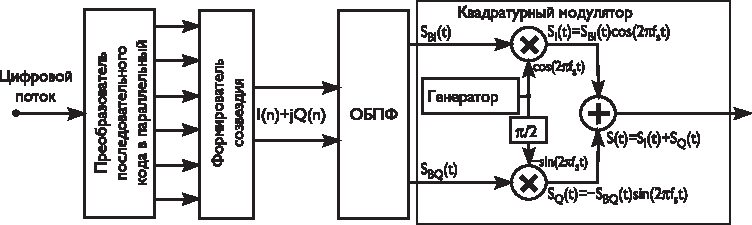
\includegraphics[width = 0.8\textwidth]{ofdm_mod_sch.pdf}
\caption{Структурная схема идеального OFDM-модулятора}
\label{ofdm_sch}
\end{figure}

На рис.~\ref{ofdm_sch} приведена структурная схема идеального OFDM-модулятора.
Цифровой поток поступает на вход преобразователя последовательной информации в параллельную.
%%%%%%%%%% ИСПРАВЛЕНИЕ %%%%%%%%%%
%На выходе этого преобразователя формируется код, состоящий из k битов и соответствующий используемой QAM-модуляции несущих ($k$ = 2 при QPSK, $k$ = 4 при QAM-16, $k$ = 6 при QAM-64 и т. д.).
На выходе этого преобразователя формируется код, состоящий из $k = \log_2N$ битов, где $N$ --- количество точек в используемом сигнальном созвездии.
%%%%%%%%%%%%%%%%%%%%%%%%%%%%%%%%%

Последовательно каждые $k$ битов преобразуются в параллельный код, который подается на формирователь созвездия, преобразующий этот код в значения соответствующих векторов звездной диаграммы.
Поток битов трансформируется в формирователе созвездия в поток I и Q сигналов:
\begin{equation}\label{eq1}
S(n) = I(n) + jQ(n),\quad 1 \leqslant n \leqslant 2N + 1,
\end{equation}
где $2N + 1 = R_a + R_n.$


Блок обратного быстрого преобразования Фурье (ОБПФ) преобразует последовательности \eqref{eq1} во временную комплексную функцию:
\begin{equation} \label{eq2}
S_B(t) = \sum_{n = 1}^{2N + 1}[I(n) + jQ(n)]exp(2\pi jnf_U t) = S_{BI}(t) + jS_{BQ}(t), 
\end{equation}
где
\[ S_{BI}(t) = \sum_{n = 1}^{2N + 1}[I(n)\cos(2\pi nf_Ut) - Q(n)\sin(2\pi nf_Ut)] \quad \mbox{--- синфазная составляющая} \]
\[ S_{BQ}(t) = \sum_{n = 1}^{2N + 1}[I(n)\sin(2\pi nf_Ut) + Q(n)\cos(2\pi nf_Ut)] \quad \mbox{--- квадратурная составляющая} \]

Связь между частотой $f_U$ и количеством несущих частот $2N + 1$ сигнала \eqref{eq2} в используемой полосе частот можно представить графиком, приведенным на рис.~\ref{ofdm2}, на котором изображены амплитуды отсчетов составляющих частот $nf_0$ ($n = 1, 2, \ldots, 2N + 1$).

\begin{figure}[h]
\centering
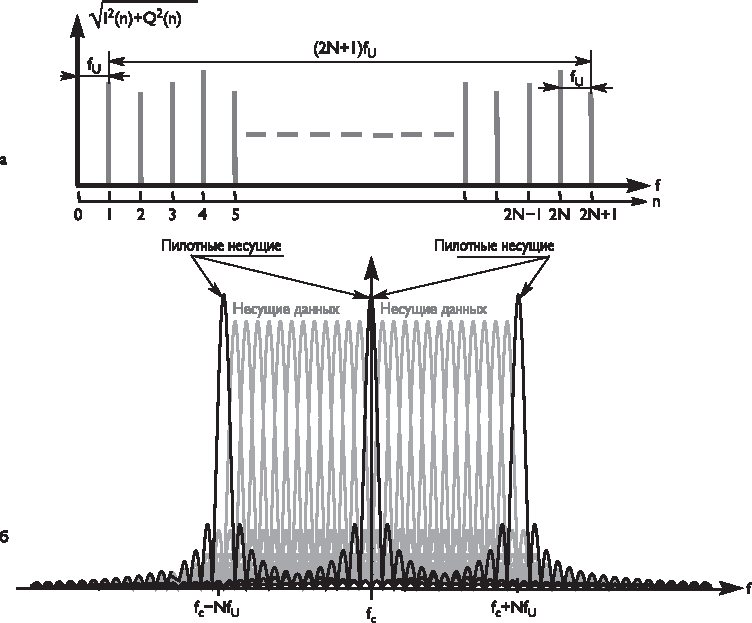
\includegraphics[width = 0.9\textwidth]{ofdm2.pdf}
\caption{График спектральных составляющих ОБПФ (а) и групповой спектр несущих частот (б)}
\label{ofdm2}
\end{figure}

В соответствии со схемой квадратурного модулятора эти два сигнала $S_{BI}(t)$ и $S_{BQ}(t)$ перемножаются соответственно на сдвинутые по фазе на $90^\circ$ синусоидальные сигналы. На выходах перемножителей формируются две составляющие:
\begin{multline}
S_I(t) = S_{BI}(t)\cdot\cos(2\pi f_st) = \sum_{n = 1}^{2N + 1}\left\{\frac{1}{2}I(n)\cdot [\cos2\pi(nf_U + f_s) + \cos2\pi(nf_U - f_s)] - \right.\\
\left.-\frac{1}{2}Q(n)\cdot [\sin2\pi(nf_U + f_s) + \sin2\pi(nf_U - f_s)]\right\},
\end{multline}
\begin{multline}
S_Q(t) = -S_{BQ}(t)\cdot\sin(2\pi f_st) = \sum_{n = 1}^{2N + 1} \left\{\frac{1}{2}I(n)\cdot [\cos2\pi(nf_U + f_s) - \cos2\pi(nf_U - f_s)] - \right.\\
\left.-\frac{1}{2}Q(n)\cdot [\sin2\pi(nf_U + f_s) - \sin2\pi(nf_U - f_s)]\right\}
\end{multline}

В результате суммирования этих двух составляющих окончательно формируется выходной сигнал OFDM-модулятора. При этом разностные частоты $nf_0 - f_s$ взаимно исключаются.

Если частота генератора $f_s$ выбрана равной $f_s = f_c + (N + 1) \cdot f_U$, где $f_c$ --- центральная частота радиоканала, то выходной сигнал определяется следующим соотношением:

\begin{multline}
S(t) = \sum_{n = 1}^{2N + 1} \left\{ I(n)\cdot\cos[2\pi(f_s + nf_U)t] - Q(n)\cdot\sin[2\pi(f_s + nf_U)t] \right\} =\\
=\sum_{n = -N}^N \left\{ I(n)\cdot\cos[2\pi(f_c + nf_U)t] - Q(n)\cdot\sin[2\pi(f_c + nf_U)t] \right\}
\end{multline}

На рис.~\ref{ofdm2}б изображена структура группового спектра несущих частот OFDM-сигнала.
Здесь условно показаны составляющие синусоидальные сигналы, промодулированные соответствующими данными созвездий дискретной QAM-модуляции.
В составе сигнала имеются также специальные пилотные несущие, на которых передается информация о параметрах системы.
Эти пилотные несущие используются также для обеспечения устойчивой синхронизации и коррекции характеристик в демодуляторе.

Таким образом, в системах с OFDM модуляцией передаваемая цифровая информация разделена на большое число низкоскоростных подканалов, длительность тактового интервала передачи каждой несущей весьма велика.
Такое построение системы преобразует широкополосный канал с одной несущей в большое число независимых узкополосных каналов с частотным разделением, что упрощает коррекцию параметров затухающего сигнала.



%\subsection{Элементы сигнала, улучшающие качество приема}
 
\subsubsection{Защитный интервал}

Ортогональность субканалов при разделении их в демодуляторе с применением БПФ может быть реализована только при отсутствии интерференции между несущими частотами, что на практике не выполняется из-за ограничения спектра и многолучевого распространения сигналов. Устранение влияния этих искажений осуществляется путем дополнения активного интервала сигнала так называемым защитным интервалом, как показано на рис.~\ref{guard}.

\begin{figure}[h]
\centering
%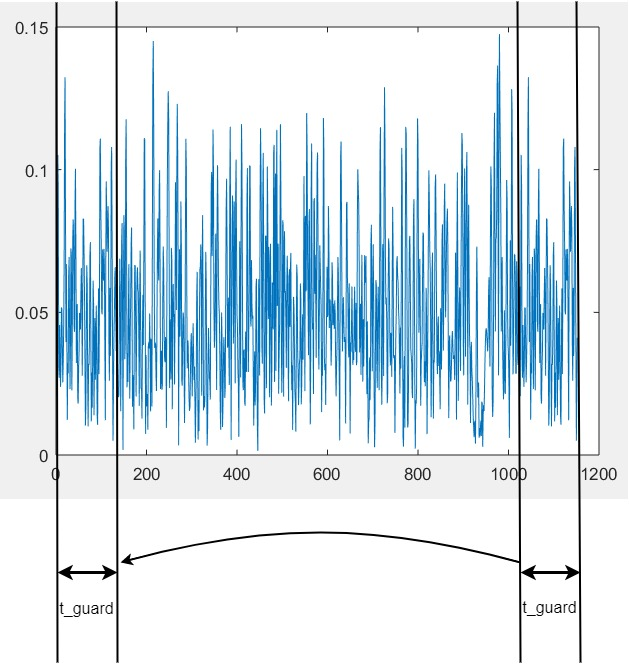
\includegraphics[width = 0.9\textwidth]{guard.pdf}
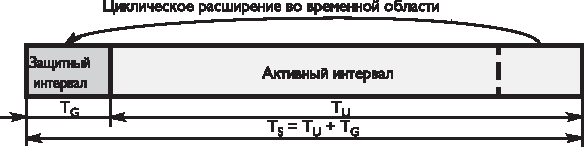
\includegraphics[width = 0.9\textwidth]{guard_a.pdf}
\caption{Формирование символа с защитным интервалом}
\label{guard}
\end{figure}

Активный интервал непрерывного символа циклически расширяется во временной области путем введения защитного интервала, содержащего часть сигнала активного интервала.
Учитывая, что на интервале $T_U$ располагается целое число периодов синусоидальных колебаний частот nfU, где $n = 1, 2, \ldots, 2N + 1$, переход от защитного интервала длительностью $T_G$ к активному интервалу не нарушает непрерывности сигнала.
Общая длительность символа сигнала OFDM оказывается равной $T_S = T_U + T_G$.

%%%%%%%%%%%% ИСПРАВЛЕНИЕ %%%%%%%%%%%%
Однако, добавление защитного интервала приводит к размыванию спектра, что ухудшает спектральную эффективность.
Это недостаток OFDM.
%%%%%%%%%%%%%%%%%%%%%%%%%%%%%%%%%%%%

%%%%%%%%%%%% ИСПРАВЛЕНИЕ %%%%%%%%%%%%
%При формировании последовательности таких символов сигнала OFDM на переходах от активного интервала предыдущего символа к защитному интервалу последующего символа возникают разрывы функций, которые в ограниченном по полосе пропускания канале преобразуются в переходные процессы, искажающие сигналы защитных интервалов.
%Для того чтобы уменьшить влияние этих переходных процессов, формируется продолжение активного интервала во временной области на некоторый интервал, по длительности равный части защитного интервала, например величине $T_G/4$, как показано на рис.~\ref{guard}б.

%Затем участки сформированных продолжений активных интервалов перемножаются на функции $u(t_1) = \cos^2\frac{\pi}{2}\frac{t_1}{T_g/4}$, где $t_1 = 0$ соответствует окончанию активного интервала, $t1 \leqslant T_G/4$, а начальные участки защитных интервалов перемножаются на функции $u(t_2) = \cos^2\frac{\pi}{2}(1 - \frac{t_2}{T_G/4})$, где $t_2 = 0$ соответствует началу защитного интервала, $t2 \leqslant T_G/4$, как отмечено на рис.~\ref{guard}б и в. 
%Непрерывный сигнал OFDM формируется путем суммирования символов рис.~\ref{guard}б и в.
%Приведенные на рис.~\ref{guard}г области переходных процессов реализуют сигналы, плавно переходящие от активных интервалов предыдущих символов к защитным интервалам текущих символов OFDM-сигналов.
%%%%%%%%%%%%%%%%%%%%%%%%%%%%%%%%%%%%

Рациональный выбор длительности защитного интервала позволяет устранить помехи, вызываемые эхосигналами, если их задержка относительно основного сигнала не превышает, скажем, половины длительности защитного интервала.



\subsubsection{Пилоты}

На приёмной стороне оценка частотного смещения на основе эталонного сигнала осуществляется с применением повторяющихся и рассеянных пилотных составляющих в OFDM-сигнале.

Повторяющиеся пилотные несущие вводятся во все без исключения OFDM-символы и занимают в них одни и те же номера поднесущих (рис.~\ref{pilots2}).
Амплитуды и фазы пилотов демодулятор использует для коррекции амплитуд и фаз активных несущих, расположенных между ними.

\begin{figure}[h]
\centering
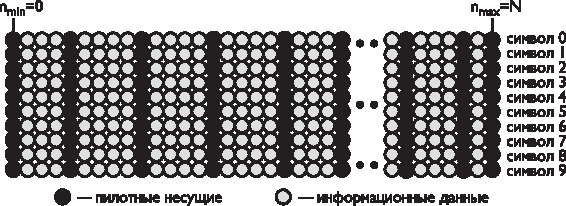
\includegraphics[width = 0.8\textwidth]{pilots2.pdf}
\caption{Повторяющиеся пилоты}
\label{pilots2}
\end{figure}

Рассеянные пилотные несущие меняют свое положение от одного OFDM-символа к другому и обычно представляются в виде диаграммы кадровой структуры, изображенной на рис.~\ref{pilots}.
%%%%%%%%%%%%% ИСПРАВЛЕНИЕ %%%%%%%%%%%%%
В этом случае в каждом OFDM-символе передаётся лишь часть пилотов (но эта часть всегда меняется от символа к символу), а освободившееся место занимают информационные несущие, что повышает скорость передачи данных.
Характеристики пропущенных пилотов в каждом символе модулятор восстанавливает по сохраненным в памяти значениям из предыдущих символов.
%%%%%%%%%%%%%%%%%%%%%%%%%%%%%%%%%%%%%%%

Краевые пилоты занимают первую и последнюю поднесущую во всех символах, при использовании как схемы с повторяющимися пилотами, так и с рассеянными.

\begin{figure}[h]
\centering
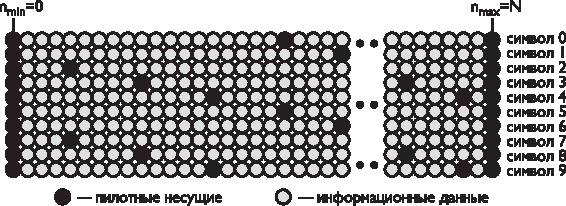
\includegraphics[width = 0.8\textwidth]{pilots.pdf}
\caption{Рассеянные пилоты}
\label{pilots}
\end{figure}

\begin{thebibliography}{9}
    \bibitem{dvorks} \textit{Дворкович В.П., Дворкович А.В.} Цифровые видеоинформационные системы (теория и практика). 2012.
    \bibitem{tanen} \textit{Танненбаум Э., Уэзерол Д.} Компьютерный сети. 5-е издание. 2012.
    \bibitem{bernard} \textit{Бернард Скляр.}
    Цифровая связь. Теоретические основы и практическое применение. 2-е издание. 2003.
    \bibitem{gonor} \textit{Гоноровский И.С.} Радиотехнические цепи и сигналы. 1986.
    \bibitem{itmo} \href{http://neerc.ifmo.ru/wiki/index.php?title=%D0%A4%D0%B8%D0%B7%D0%B8%D1%87%D0%B5%D1%81%D0%BA%D0%B8%D0%B9_%D1%83%D1%80%D0%BE%D0%B2%D0%B5%D0%BD%D1%8C_-_%D0%9C%D0%BE%D0%B4%D1%83%D0%BB%D1%8F%D1%86%D0%B8%D0%B8}{http://neerc.ifmo.ru/wiki/index.php?title=Физический\_уровень\_-\_Модуляции}
\end{thebibliography}




%\graphicspath{{./}}  % возвращение к исходной папке
